\documentclass[a4paper,11pt]{article}


%% Language and font encodings
\usepackage[english]{babel}
\usepackage[utf8x]{inputenc}
\usepackage{colortbl}
\usepackage[T1]{fontenc}

%% Sets page size and margins
\usepackage[a4paper,top=3cm,bottom=2cm,left=3cm,right=3cm,marginparwidth=1.75cm]{geometry}

%% Useful packages
\usepackage{amsmath}
\usepackage{graphicx}
\usepackage[colorinlistoftodos]{todonotes}
\usepackage[colorlinks=true, allcolors=blue]{hyperref}

\title{Final Report}
\author{Written by : GoChat Team}

\begin{document}
\maketitle

%\begin{abstract}
%Your abstract.
%\end{abstract}

\section{Introduction}





%WebSocket Protocol is used to ensure the communication between clients and server. (The WebSocket is a feature of HTML5 for establishing a socket connections between a web browser and a server, once the connection has been established with the server, all WebSocket data (frames) are sent directly over a socket rather than usual HTTP response and requests, giving us much faster, persistent and full-duplex communication between a web browser and a server.)





%\subsection{Project Scope}



\section{Review}

\section{Requirement and Design}



\subsection{Requirement}
The requirement for this project is to build a reliable, secure, and attractive chat system. Reliable in the term that every message sent by the client will receive in a relatively real-time. The client would not have to concern about lost message even in a slow network connection or offline case. Meanwhile, secure in this case means that there is no unauthorized principal can read a message sent from one client to another client.

According to the requirement, we divided our project into three main level, Basic Chatting Program, Security, and Other Additional Functions. 
\subsubsection{Level 1: Basic Functionalities}
In this level, basic infrastructure will be built for the server and two clients, the web page and the Windows desktop application, to achieve basic functionalities for the system. 

\begin{itemize}
%--------------------------------------------------------
%change User




\item Server
\begin{enumerate}
\item The database is used to store users' names, passwords, personal information, friends' information and chatting information in the server.
\item Apache server is used to make a connection between server and clients.
\end{enumerate}


%: Keep chatting record in the database. It store data until the user request to delete history.

%: describe database table(how to store data)

%: it might be depend on option. If someone do not want to store data(like private mode), data will delete when user delete chatting.

% : open web sever by open source program Apache

% : it can be replace by github(github provide storage. it can use as a web server)


\item Client
\begin{enumerate}
\item Clients could set up the connection with server (Figure 2).
\item Client 1 sends message to server
\item Client 2 receive the message from the server which from the client 1.
\item If the message is not a plain text, client 2 send a request to the server to receive data.
\item Client 2 receive data which as picture and document.
\end {enumerate}
\item User

\begin{enumerate}
\item Users on the clients could sign up creating their usernames and passwords and also filling in their personal details.
\item Users on the clients could add their friends and send messages (text, files and pictures) to them.
\item Users on the clients could check whether their friends are online or not.
\item  Users on the clients could create groups with adding their friends to the group and begin group chats.

\end{enumerate}
\end{itemize}
\begin{figure}[h]
\centering
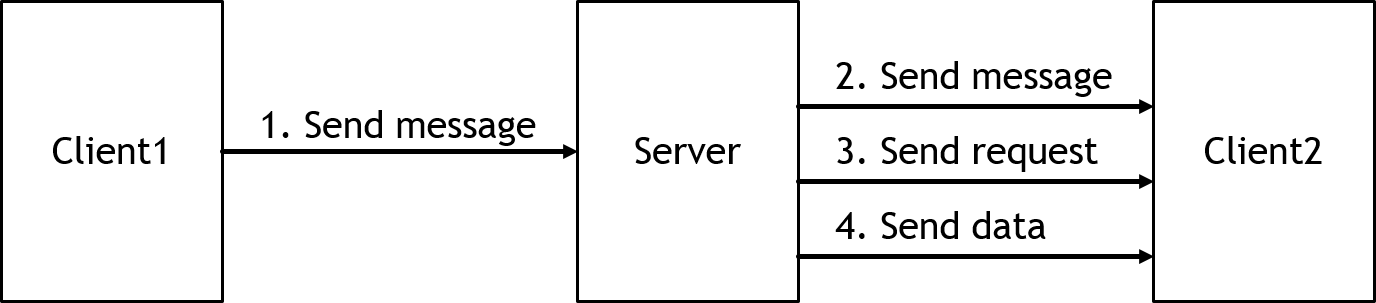
\includegraphics[width = 0.6 \textwidth ]{client_server.png}
\caption{\label{fig:UML2}Server/Client Model}
\end{figure}
%\begin{table}[h]
%\caption{Payload}
%\begin{center}
%\begin{tabular}{| c | c | c | c |}
%\hline
%sender & receiver & type & message\\
%\hline
%\end{tabular}
%\end{center}
%\end{table}

% \begin{itemize}
% \item Payload

% - This is a simple version of the payload for communicating between server and client

% - type: provide what type of the message it is. Such as plain text, picture, video, and document.

% - message: If message is a plain text, it contains the text. Another cases (picture, and so on), it contains server storage a URL. Based on the URL, files will be download from the server. 

% \end{itemize}
\subsubsection{Level 2: Security}

Chatting program is a private communication. Confidentiality, Privacy, and Integrity are common issues at the chatting program. It contains personal information, photos, business secret, and so on. This kind of information must be encrypted to avoid leakage. For encryption, many solutions are available such as trusted third party protocol or asymmetric keys encryption.

While level 1 provides basic functionalities without considering the security, the aim of the go-chat level 2 is to keep everything secure. In level 1, program store unencrypted history at the server. Meanwhile, in level 2, it will be encrypted by security protocols, so that only those who participate in the chatting can read their chatting history. In this level, the user also should be able to delete their chatting history to prevent data theft. In addition, user can customise message expire time. For example, if user set the expire time to one day, the message will be automatically deleted after 24 hours. The message will be deleted even if the receiver has not seen the message.

In term of security aspect, we will focus on two parts, communication security and security of data storage. For communication security, WebSocket protocol doesn’t handle the authorization or authentication. However, just like the HTTPs which is HTTP over TLS, using the WSS (WebSocket over TLS/SSL) to encrypt our connection can make sure our information transfer security. In this case, we just need to configure TLS encryption for WebSocket and self-sign the certificate. For database security, we choose to use SALT and hash function to encrypt the username and password to avoid dictionary attacks. Using different encryption algorithm is for other data. In this way, we can prevent the SQL injection attack.

\subsubsection{Level 3: Other Additional Functionalities}

Chatting program has to be attractive. It is not only for sending plaintext messages to friends. It has to be possible to express emotion of people. That's why people use emojis and photos. In level 3 period, go-chat program contain attractive function including using emojis, gif, drawing picture, recommending friend, offline message, printing history, recalling the message, and image compose.
\subsection{Design}
\subsubsection{Project Structure}
\begin{figure}[h]
\centering
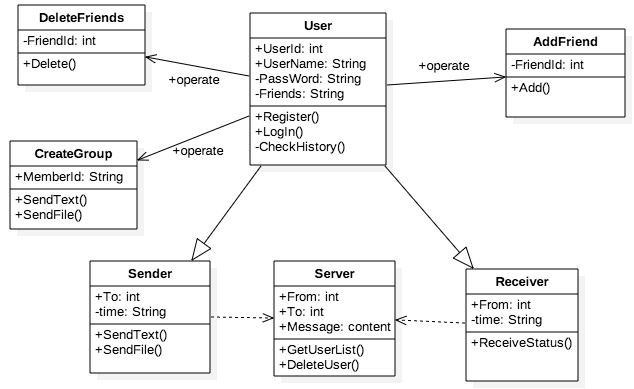
\includegraphics[width = 0.8 \textwidth ]{UML.png}
\caption{\label{fig:UML}UML Class Diagram}
\end{figure}




%-----------------------------------------------
% add some description 




Since storing chat messages and retrieving those messages at a very fast rate is much needed for a chatting software, the MYSQL is used as our database management system, and four tables will be created to store different sorts of data.


\begin{figure}[h]
\centering
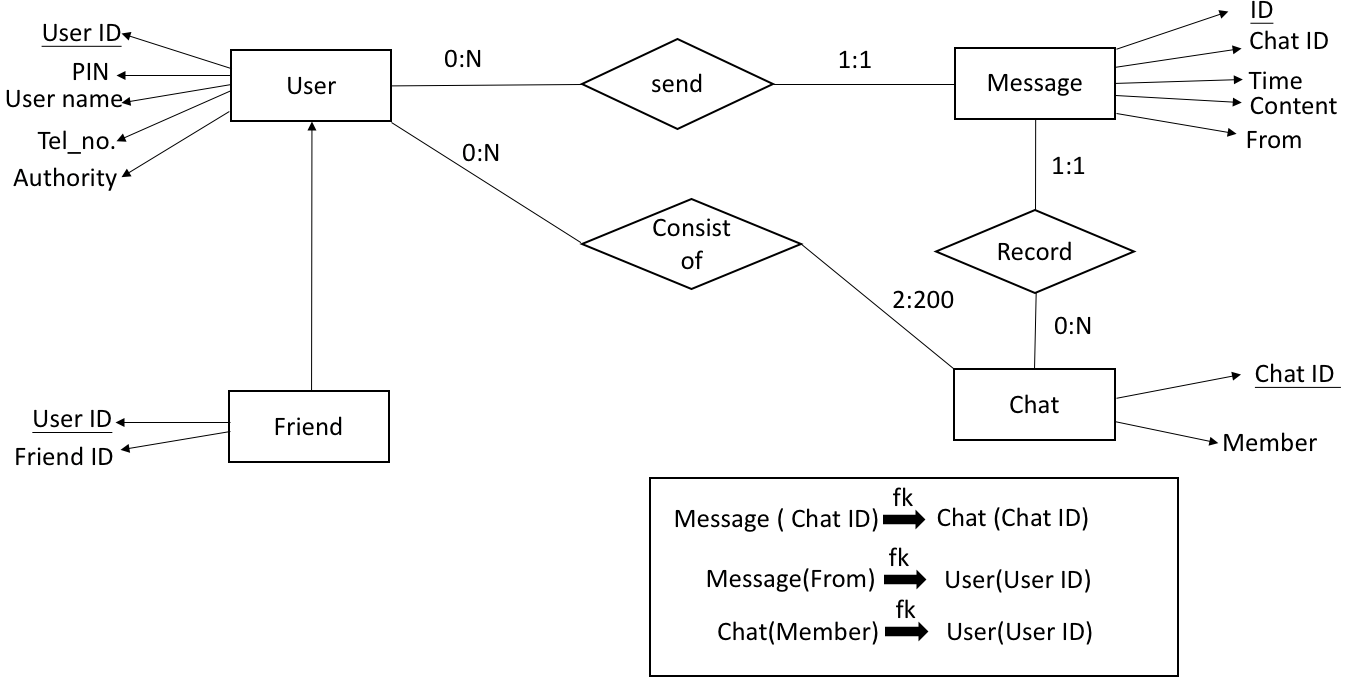
\includegraphics[width = 0.8 \textwidth ]{ERD.png}
\caption{\label{fig:ERD}Entity Relation Diagram}
\end{figure}

\begin{itemize}
\item Table ‘user’ would contain the basic information of all users including userID, password, username, etc. 
\item Table ‘friend’ is used to store the userID and the friendID of their friends’.
\item Table ‘message’ will list the detail of every single message including chatID, sending time, a content of the message, and the sender’s userID.
\item Table ‘chat’ is used to record the member of chatting and their chatID. 
\end{itemize}


\begin{itemize}
\item Key constraint:

Primary key: user(userID), message(ID), friend(userID), chat(chatIÅD).

Foreign key: message(chatID), message(from), chat(member).

\end{itemize}

\section{Implementation}
\subsection{Window Desktop Client}
\subsubsection{UI Design}
There are three forms constituting the Gochat windows desktop application, login form (Figure), sign up form (Figure) and chat form (Figure). In login form, existing users could type user name and password to login while new users could click sign up button to sign up in sign up form. In sign up form, users could choose their profile photos from local folders, user names and passwords. 
After users login, the chat form will show out. It is shown in Figure that chat form is divided into three parts, control panel providing buttons for users to add friends, create groups and sign out, list section and message window. In the list section, users can see friend list, group list and chat list by click different buttons. When users click a friend, a group or a chat from the list section, all chatting history will display in message window. Also, on the bottom of the message window, users could type and send the messages. On the top, images or files could be sent as well by clicking the corresponding picture buttons. 
\subsubsection{List and Message Display}
User control item named chatmesg is embedded into another user control item called chatbox to display every single message. When new message is sent or received, new user control item will be generated and displayed below the preview ones. Chatmesg, textbox, send message button, select image and file buttons are combined together in chatbox user control item and embedded into chat form. Likewise, user control item, friend item is used to display each friend or chat or group in the list section and also embedded into friend list user control item. The friend list user control item is embedded into chat form at the end.   
 
\subsubsection{Send and receive message or Images or Files}
\section{Evaluation}
\subsection{Level 1}
 
\subsubsection{Server}

With more researches about Apache server going on, we found out that Apache server can not communicate with window client. And then, we tried to design a window desktop server instead according to demonstrations and references found online. But after having the server running, we found out the web client can not receive messages from the server continuously. While spending time to solve the problem in the window desktop server, we were also doing researches about web server.   Since the window desktop server problem can not be fixed and a web server used Javascript as programming language achieved our goal, communicating with both window client and web client using WebSocket protocol, the web server was built and chose at the end.  

 
\subsubsection{Clients}
The client part is slightly changed. When client 1 sends files or images, the client will firstly send file path in a given format to the server. By the meantime, the file is uploaded to the specific folder in the server. After that, the server will send the file path to client 2.

\subsection{Level 2}
Due to the limitation of time, the function that users could delete their chatting history and customize their chatting history expire time to prevent data theft has not been done. 


In communication security part, Elliptic curve Diffie-Helmen key exchange and AES key encryption is used because of time limitation. 

\subsection{Level3}
Due to the limitation of time, level 3 has not been done.

\subsection{Time management}

\definecolor{No}{RGB}{255,255,185}
\definecolor{UML}{RGB}{205,205,180}
\definecolor{Data}{RGB}{205,205,180}
\definecolor{intermediate}{RGB}{205,205,180}
\definecolor{environ}{RGB}{205,205,180}
\definecolor{level1}{RGB}{205,205,180}
\definecolor{level2}{RGB}{205,205,180}
\definecolor{level3}{RGB}{205,205,180}
\definecolor{debug}{RGB}{205,205,180}
\definecolor{documentation}{RGB}{205,205,180}
\definecolor{final}{RGB}{205,205,180}
\begin{table}[h]
\centering
\caption{Task time table (Initial)}
\label{my-label}
\begin{tabular}{|c|l||c|c|c|c|c|c|c|c|c|c|}
\hline
\rowcolor{No}
No. & Task name & 01 & 02 & 03 & 04 & 05 & 06 & 07 & 08 & 09 & 10 \\ \hline \hline
1 & UML design & \cellcolor{UML} & \cellcolor{UML} &  &  &  &  &  &  &  &  \\ \hline
2 & Database design & \cellcolor{Data} & \cellcolor{Data} &  &  &  &  &  &  &  &  \\ \hline
3 & Intermediate report \& presentation &  & \cellcolor{intermediate} & \cellcolor{intermediate} &  &  &  &  &  &  &  \\ \hline
4 & Developing environment setting &  &  & \cellcolor{environ} & \cellcolor{environ} &  &  &  &  &  &  \\ \hline
5 & Level 1: basic chatting program &  &  & \cellcolor{level1} & \cellcolor{level1} & \cellcolor{level1} &  &  &  &  &  \\ \hline
6 & Level 2: security &  &  &  &  & \cellcolor{level2} & \cellcolor{level2} & \cellcolor{level2} &  &  &  \\ \hline
7 & Level 3: Other additional function &  &  &  &  &  &  & \cellcolor{level3} & \cellcolor{level3} & \cellcolor{level3} &  \\ \hline
8 & Debug &  &  &  &  & \cellcolor{debug} & \cellcolor{debug} & \cellcolor{debug} & \cellcolor{debug} & \cellcolor{debug} & \cellcolor{debug} \\ \hline
9 & Documentation &  &  &  &  & \cellcolor{documentation} &  & \cellcolor{documentation} &  & \cellcolor{documentation} &  \\ \hline
10 & Final report \& presentation &  &  &  &  &  &  &  &  & \cellcolor{final} & \cellcolor{final} \\ \hline
\end{tabular}
\end{table}

\definecolor{No}{RGB}{255,255,185}
\definecolor{UML}{RGB}{205,205,180}
\definecolor{Data}{RGB}{205,205,180}
\definecolor{intermediate}{RGB}{205,205,180}
\definecolor{environ}{RGB}{205,205,180}
\definecolor{level1}{RGB}{205,205,180}
\definecolor{level2}{RGB}{205,205,180}
\definecolor{level3}{RGB}{205,205,180}
\definecolor{debug}{RGB}{205,205,180}
\definecolor{documentation}{RGB}{205,205,180}
\definecolor{final}{RGB}{205,205,180}
\begin{table}[h]
\centering
\caption{Task time table (Last)}
\label{my-label}
\begin{tabular}{|c|l||c|c|c|c|c|c|c|c|c|c|}
\hline
\rowcolor{No}
No. & Task name & 01 & 02 & 03 & 04 & 05 & 06 & 07 & 08 & 09 & 10 \\ \hline \hline
1 & UML design & \cellcolor{UML} & \cellcolor{UML} &  &  &  &  &  &  &  &  \\ \hline
2 & Database design & \cellcolor{Data} & \cellcolor{Data} &  &  &  &  &  &  &  &  \\ \hline
3 & Intermediate report \& presentation &  & \cellcolor{intermediate} & \cellcolor{intermediate} &  &  &  &  &  &  &  \\ \hline
4 & Developing environment setting &  &  & \cellcolor{environ} & \cellcolor{environ} &  &  &  &  &  &  \\ \hline
5 & Level 1: basic chatting program &  &  & \cellcolor{level1} & \cellcolor{level1} & \cellcolor{level1} &  &  &  &  &  \\ \hline
6 & Level 2: security &  &  &  &  & \cellcolor{level2} & \cellcolor{level2} & \cellcolor{level2} &  &  &  \\ \hline
7 & Level 3: Other additional function &  &  &  &  &  &  & \cellcolor{level3} & \cellcolor{level3} & \cellcolor{level3} &  \\ \hline
8 & Debug &  &  &  &  & \cellcolor{debug} & \cellcolor{debug} & \cellcolor{debug} & \cellcolor{debug} & \cellcolor{debug} & \cellcolor{debug} \\ \hline
9 & Documentation &  &  &  &  & \cellcolor{documentation} &  & \cellcolor{documentation} &  & \cellcolor{documentation} &  \\ \hline
10 & Final report \& presentation &  &  &  &  &  &  &  &  & \cellcolor{final} & \cellcolor{final} \\ \hline
\end{tabular}
\end{table}



\subsection{Future Work}











\end{document}
